\section{宇宙膨胀的动力学}\label{sec:05.05}

前面证明宇宙膨胀时,实际上只用到牛顿运动学的知识,现
在我们来讨论它的动力学性质。

由于膨胀是均匀的,我们只要研究一些典型天体的运动,就
% 162.jpg
\clearpage\noindent
可以得知膨胀运动的全貌。我们选一个以$ O $为心的球壳上的星体,
这组星体相对于$ O $不断地膨胀,但始终保持球壳的形状。

设在$ t $时刻,若在$ \vec{r}_0 $(单位矢量)方向的球壳上的星体位于$ \vec{r} $,
则可以表为
\begin{equation}\label{eqn:05.05.01}
  \vec{r} = R \left( t \right) \vec{r} _ { 0 }
\end{equation}
其中$ R\left(t\right) $称为宇宙尺度因子,它描写这个球壳的尺度。

按速度的定义,有
\begin{equation}\label{eqn:05.05.02}
  \vec{q} = \frac { \dif \vec{r} } { \dif t }
\end{equation}
将式\eqref{eqn:05.05.01}及式\eqref{eqn:05.05.02} 代入式\eqref{eqn:05.03.05},得
\begin{equation}\label{eqn:05.05.03}
  \frac { \dif R } { \dif t } = f \left( t \right) \cdot R \left( t \right)
\end{equation}

现在研究位于$\vec{r}$的质点(或星体)$ P $相对于$ O $的运动方程。按
\begin{wrapfigure}[9]{r}{10em}
  \centering
  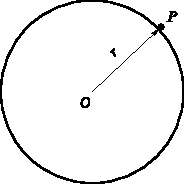
\includegraphics{figure/fig05.04}
  \caption{宇宙膨胀的动力学}
  \label{fig:05.04}
\end{wrapfigure}
牛顿引力理论,以$ O $为中心,$ |\vec{r}| $为半径的
球体内的质量对$ P $有吸引力(图\ref{fig:04.10}),
引力的强度是
\begin{equation*}
  G \frac { 4 \uppi } { 3 } R ^ { 3 } \rho / R ^ { 2 } = G \frac { 4 \uppi } { 3 } R \rho
\end{equation*}
其中$ \rho $为宇宙间的平均密度,引力的方
向沿着$ - \vec{r} _ 0 $。另一方面,因为分布是对
称的,$ OP $球之外的天体对$ P $的作用为
零。这样$ P $点的动力学方程为
\begin{equation*}
  \frac { \dif ^ { 2 } \vec{r} } { \dif t ^ { 2 } } = - \frac { 4 \uppi G } { 3 } R \rho \vec{ r } _ 0
\end{equation*}
将式\eqref{eqn:05.05.01}代入上式得
\begin{equation*}
  \frac { \dif ^ { 2 } R } { \dif t ^ { 2 } } \vec{r} _ { 0 } = - \frac { 4 \uppi G } { 3 } R \rho \vec{r} _ 0
\end{equation*}

% 163.jpg
\clearpage\noindent
或
\begin{equation}\label{eqn:05.05.04}
  \frac { \dif ^ { 2 } R } { \dif t ^ { 2 } } = - \frac { 4 \uppi G } { 3 } R \rho
\end{equation}

在求解式\eqref{eqn:05.05.04}时,我们应当注意到,在膨胀或收缩过程
中,球壳内的总质量是不变的,因此,有
\begin{equation*}
  \rho R ^ { 3 } = \text{常数}
\end{equation*}
或
\begin{equation}\label{eqn:05.05.05}
  \rho R ^ { 3 } = \rho _ 0 { R _ 0} ^ { 3 }
\end{equation}
其中$ \rho _ { 0 } $及$ R _ 0 $分别是$ t _ { 0 } $时刻的平均密度及宇宙尺度因子,将式
\eqref{eqn:05.05.05}代入式\eqref{eqn:05.05.04},得到
\begin{equation}\label{eqn:05.05.06}
  \frac { \dif ^ { 2 } R } { \dif t ^ { 2 } } = - \frac { 4 \uppi G } { 3 } \cdot \frac { \rho _ { 0 } R _ { 0 } ^ { 3 } } { R ^ { 2 } }
\end{equation}
将上式两边乘以$ \dfrac { \dif R } { \dif t } $,并注意下列关系
\begin{equation*}
  \begin{aligned}
    \frac { \dif R } { \dif t } \cdot \frac { \dif ^ { 2 } R } { \dif t ^ { 2 } }
     & = \frac { 1 } { 2 } \cdot \frac { \dif } { \dif t } \left( \frac { \dif R } { \dif t } \right) ^ { 2 } - \frac { 4 \uppi G } { 3 } \rho _ { 0 } R _ { 0 } ^ { 3 } \frac { 1 } { R ^ { 2 } } \cdot \frac { \dif R } { \dif t } \\
     & = \frac { 4 \uppi G } { 3 } \rho _ { 0 } R _ 0 ^ { 3 } \frac { \dif } { \dif t } \left( \frac { 1 } { R } \right)
  \end{aligned}
\end{equation*}
则可得到
\begin{equation*}
  \frac { \dif } { \dif t } \left[ \frac { 1 } { 2 } \left( - \frac { \dif R } { \dif t } \right) ^ { 2 } - \frac { 4 \uppi G } { 3 } \rho _ { 0 } P _ { 0 } ^ { 3 } \frac { 1 } { R } \right] = 0
\end{equation*}
积分后得到
\begin{equation}\label{eqn:05.05.07}
  \left[ \frac { 1 } { R _ { 0 } } \left( \frac { \dif R } { \dif t } \right) \right] ^ { 2 } - \frac { 8 \uppi G } { 3 } \rho _ 0 \frac { 1 } {\left( \dfrac { R } { R _ { 0 } }\right)} = K
\end{equation}
其中$ K $表示积分常数,我们分以下两种花况讨论式\eqref{eqn:05.05.07}。

(1) $ K > 0 $时,由式\eqref{eqn:05.05.07}得到
\begin{equation}\label{eqn:05.05.08}
  \frac { \dif R } { \dif t } = \pm \sqrt { \frac { 8 \uppi G } { 3 } \rho _ { 0 } R _ { 0 } ^ { 3 } \frac { 1 } { R } + K R _ 0 ^ { 2 } }
\end{equation}
其中正号表示膨胀运动,负号表示收缩运动。由于根号下的量对
% 164.jpg
任何大的$ R $值总是正的,所以,这种情况的结论是,一旦宇宙处
胀状态,则无论$ R $膨胀到多大,总有$ \dfrac { \dif R } { \dif t } > 0 $,即总处在膨
胀状态。这称为无限膨胀解。

(2) $ K < 0 $时,代替式\eqref{eqn:05.05.08},则有
\begin{equation}\label{eqn:05.05.09}
  \frac { \dif R } { \dif t } = \pm \sqrt { \frac { 8 \uppi G } { 3 } \rho _ { 0 } R _ { 0 } ^ { 3 } \frac { 1 } { R } - | K | R _ 0 ^ { 2 } }
\end{equation}
因此,当宇宙膨胀到
\begin{equation}\label{eqn:05.05.10}
  R = R _ { \text { max } } \equiv \frac { 8 \uppi G } { 3 } \rho _ { 0 } R _ { 0 } ^ { 3 } \frac { 1 } { | K | R _ { 0 } ^ 2 }
\end{equation}
有
\begin{equation*}
  \frac { \dif R } { \dif t } = 0
\end{equation*}
即膨胀停止。而且,对于$ R > R _ { \text { max } } $ 范围,式\eqref{eqn:05.05.09}的根式成为虚数,
故不是物理解。这说明,宇宙不可能膨胀到$ R > R _ { \text { max } } $范围。因此,
在这种情况的结论是,宇宙膨胀到$ R = R _ { \text { max } } $,转变为收缩,这称
为膨胀-收缩解。

总之,我们的宇宙可能有两种前景,一是将永远膨胀下去,
一是将来会停止膨胀,并变成收缩。到底是哪一种前景,将取决
于$ K $的符号。

由于方程\eqref{eqn:05.05.07}对任何时刻都成立,我们取$ t=t_0 $时刻,则
有
\begin{equation}\label{eqn:05.05.11}
  K = \left[ \frac { 1 } { R _ { 0 } } \left( \frac { \dif R } { \dif t } \right) _ 0 \right] ^ { 2 } - \frac { 8 \uppi G } { 3 } \rho _ { 0 }
\end{equation}
其中$ R _ { 0 } = R \left( t _ { 0 } \right) $。另外,由式\eqref{eqn:05.05.03},得
\begin{equation*}
  \frac { 1 } { R _ { 0 } } \left( \frac { \dif R } { \dif t } \right) _ { 0 } = f \left( t _ { 0 } \right) = H _ { 0 }
\end{equation*}
所以,式\eqref{eqn:05.05.11}可变成
\clearpage
% 165.jpg
\begin{equation}\label{eqn:05.05.12}
  K = H _ 0 ^ { 2 } - \frac { 8 \uppi G } { 3 } \rho _ { 0 }
\end{equation}
定义下列量
\begin{equation*}
  \rho _ { c } \equiv \frac { 3 H _ 0 ^ { 2 } } { 8 \uppi G } \approx 4.8 \times 10 ^ { -30 } \text{克/厘米} ^ 3
\end{equation*}
它称为临界质量密度。由式\eqref{eqn:05.05.12}可得

(1)当$ \rho _ { 0 } < \rho _ { c } $时,$ K > 0 $;

(2)当$ \rho _ { 0 } > \rho _ { c } $时,$ K < 0 $。

\noindent 所以,我们宇宙的前景,完全决定于现今(即$ t _ { 0 } $时刻)宇宙中的平
均质量密度$ \rho _ { 0 } $。目前对$ \rho _ { 0 } $的测量还十分不准确,尚不清楚$ \rho _ { 0 } $是
大于或小于临界密度$ \rho _ { c } $。这是现代宇宙学正在研究的一个问题。
